\documentclass[english,notitlepage]{article}  % defines the basic parameters of the document
\usepackage[T1]{fontenc} %for å bruke æøå
\usepackage[utf8]{inputenc}
\usepackage{graphicx} %for å inkludere grafikk
\usepackage{mathpazo}
\usepackage[norsk]{babel}
% Standard stuff
\usepackage{amsmath,graphicx,varioref,verbatim,amsfonts,geometry,gensymb, multirow}
% colors in text
\usepackage[usenames,dvipsnames,svgnames,table]{xcolor}
% Hyper refs
\usepackage[colorlinks=true,allcolors=black]{hyperref}

\usepackage{caption}
\usepackage{enumitem}
\usepackage{tikz}             % draw figures manually
\usepackage{subfigure}        % imports a lot of cool and useful figure commands
\usepackage{float}
\usepackage{circuitikz}
\usepackage{listings}

\usepackage{csquotes}
\usepackage[backend=biber,style=alphabetic,sorting=ynt]{biblatex} %Imports biblatex package
\addbibresource{referanser.bib}

\title{FYS3150\\Project 2}
\author{Brage A. Trefjord\\Sigurd Sønvisen Vargdal\\Frida Oleivsgard Sørensen\\Nils Enric Canut Taugbøl}


\begin{document}

\maketitle
\textit{GitHub repository:} \texttt{\url{https://github.com/NilsECT/FYS3150/tree/main/Project_2/Code}}


\section*{Problem 1:}

We use the dimensionless variable $\hat{x} = \frac{x}{L}$, which gives us
$\frac{d \hat{x}}{dx} = \frac{1}{L}$. Using this, we get:

\begin{align*}
    \frac{d}{dx} = \frac{d\hat{x}}{dx} \frac{d}{d\hat{x}} = \frac{1}{L} \frac{d}{d\hat{x}}
\end{align*}

And we can find the scaled differential equation:

\begin{align*}
    \gamma \frac{d^2 u(x)}{dx^2} &= -F u(x)
    \\
    \gamma \left( \frac{1}{L} \frac{d}{d\hat{x}} \right)^2 u(\hat{x}) &= -F u(\hat{x})
    \\
    \gamma \frac{1}{L^2} \frac{d^2 u(\hat{x})}{d \hat{x}^2} &= -F u(\hat{x})
    \\
    \frac{d^2 u(\hat{x})}{d \hat{x}^2} &= - \frac{F L^2}{\gamma} u(\hat{x})
    \\
    \frac{d^2 u(\hat{x})}{d \hat{x}^2} &= - \lambda u(\hat{x}) \; , \hspace*{20pt} \lambda \equiv \frac{F L^2}{\gamma}
\end{align*}


\section*{Problem 2}

Our tridiagonal $6 \times 6$ matrix is

\begin{equation*}
    A = \frac{1}{h^2} \begin{bmatrix}
        2 & -1 & 0 & 0 & 0 & 0 \\
        -1 & 2 & -1 & 0 & 0 & 0 \\
        0 & -1 & 2 & -1 & 0 & 0 \\
        0 & 0 & -1 & 2 & -1 & 0 \\
        0 & 0 & 0 & -1 & 2 & -1 \\
        0 & 0 & 0 & 0 & -1 & 2
    \end{bmatrix}
\end{equation*}

where $h = \frac{1}{N+1}$, and $N = 6$ is the dimension of our square matrix.

We solve the equation

\begin{equation*}
    A \vec{v} = \lambda \vec{v}
\end{equation*}

both analytically and using armadillo in C++. Here $\lambda$ are the
eigenvalues, and $\vec{v}$ are the corresponding eigenvectors of $A$. See code
in repository. We find that the eigenvectors from armadillo are consistent with
those found analytically.


\section*{Problem 3}
\subsection*{a)}
See code in repository.

\subsection*{b)}
To test the solving method we write a program generating the test matrix. We use Armadillos eigsym to test against. The code sortes the eigenvectors in order of raising eigenvalue. Then checks if the two matrices are equal with a tolerance of $1e-7$. The code prints a statment telling us if the two matrices are equal.

\section*{Problem 4}

See code in repository.


\section*{Problem 5}
\subsection*{a)}
(See code in repository.)\\
We have an $N \times N$ tridiagonal matrix. 

\begin{figure}[H]
    \centering
    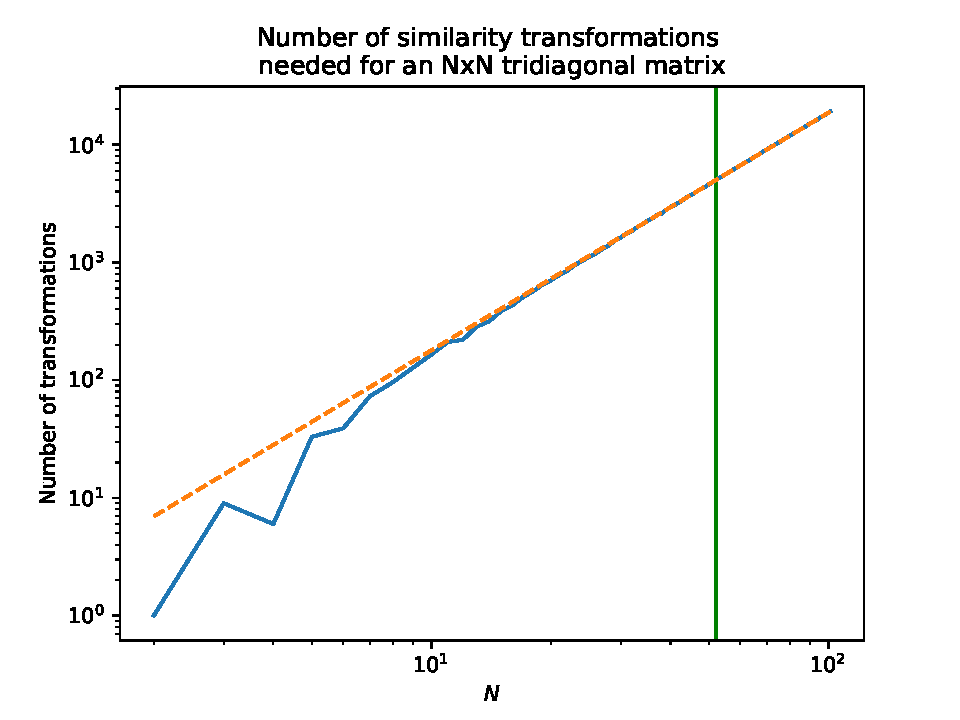
\includegraphics[width=0.8\linewidth]{../Code/Problem_5_plot.pdf}
    \caption{Loglog plot of the number of transformations needed to compute the eigen values for an $N \times N$ matrix with a tolerance of 1e-10.}
    \label{fig:5plot}
\end{figure}

\subsection*{b)}
For a Dense matrix we expect.. scaling behavior.

\section*{Problem 6}
\subsection*{a)}
See code in repository.

\begin{figure}[H]
    \centering
    \includegraphics[width=0.8\linewidth]{../Code/Problem_6_a_plot.pdf}
    \caption{Plot of the 3 lowest eigen vectors with the boundary conditions 0 at the start and the beginning for $n=10=>N=9$.}
    \label{fig:6aplot}
\end{figure}

\subsection*{b)}

\begin{figure}[H]
    \centering
    \includegraphics[width=0.8\linewidth]{../Code/Problem_6_b_plot.pdf}
    \caption{Plot of the 3 lowest eigen vectors with the boundary conditions 0 at the start and the beginning for $n=100=>N=99$.}
    \label{fig:6bplot}
\end{figure}

\end{document}